\section{Models and Experimental Controls}
\label{sec:method}

\begin{figure*}[!t]
\centering\resizebox{\textwidth}{!}{\begin{tikzpicture}[
  x=1cm,y=1cm,
  flow/.style={draw=aegisgray!35,fill=aegishead,
    text width=3.6cm,minimum height=1.38cm,inner sep=4pt,align=center,font=\small},
  study/.style={draw=aegisblue!30,fill=aegisbest,
    text width=4.95cm,minimum height=1.24cm,inner sep=4pt,align=center,font=\small},
  arrow/.style={-{Latex[length=2.1mm]},aegisblue,line width=.75pt}
]
\node[flow] (sources) at (1.96,0) {\textbf{Paired weather data}\\Rain, fog, snow, smoke};
\node[flow] (split) at (6.35,0) {\textbf{Training and validation}\\18,610 train pairs\\2,011 validation pairs};
\node[flow] (train) at (10.74,0) {\textbf{Train six restorers}\\Select checkpoints by\\validation PSNR};
\node[flow] (test) at (15.13,0) {\textbf{Held-out comparison}\\2,334 test pairs\\Balanced PSNR and SSIM};
\draw[arrow] (sources) -- (split);
\draw[arrow] (split) -- (train);
\draw[arrow] (train) -- (test);
\node[draw=aegisblue!45,fill=aegisblue!8,inner xsep=10pt,
      inner ysep=4pt,font=\small\bfseries] (checkpoint) at (8.55,-1.70)
      {Trained Restormer checkpoint (epoch 51)};
\draw[arrow] (train.south) |- (checkpoint.east);
\node[study] (joint) at (2.68,-3.32) {\textbf{Continuation study}\\Eight arms from the same weights\\Matched training control};
\node[study] (dawn) at (8.55,-3.32) {\textbf{Downstream detection}\\Local controls and labelled Nano\\Frozen YOLOv8n};
\node[study] (edge) at (14.42,-3.32) {\textbf{Edge measurements}\\Nano throughput and input energy\\Separate compression screens};
\coordinate (branch) at (8.55,-2.37);
\draw[aegisblue,line width=.75pt] (checkpoint.south) -- (branch);
\draw[arrow] (branch) -| (joint.north);
\draw[arrow] (branch) -- (dawn.north);
\draw[arrow] (branch) -| (edge.north);
\end{tikzpicture}
}
\caption{Shared workflow from paired images to model and deployment evaluation. Training and validation select one checkpoint per model. The held-out split supplies the six-model comparison. The trained epoch-51 Restormer initializes the continuation arms, supplies the restored DAWN views, and is exported for the device evaluation.}
\label{fig:project-workflow}
\end{figure*}

\begin{figure*}[!t]
\centering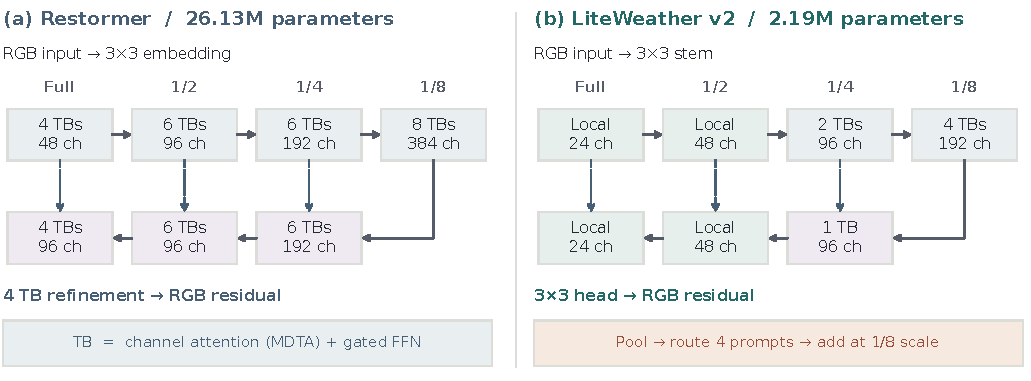
\includegraphics[width=\textwidth]{figures/restorer_architectures.pdf}
\caption{Architectures evaluated on the paired benchmark. Restormer uses transformer blocks (TBs) at all four scales. LiteWeather v2 uses local residual blocks at full and half resolution and attention at quarter and eighth resolution. Its soft prompt mixture is added before the eighth-scale transformer blocks. Arrows between scales represent down/up-sampling. Dashed arrows show encoder-to-decoder concatenation. Each network predicts a residual added to the degraded RGB image.}
\label{fig:architecture}
\end{figure*}

\paragraph{Shared training schedule.}
All six recipes use seed 42, 60 epochs, global batch four, and 4,096 paired draws per epoch with random $256\times256$ crops and flips. Background-aware sampling with replacement uses rain/fog/snow/smoke probabilities of 0.30/0.30/0.30/0.10. The non-GAN runs use L1 and AdamW, a $10^{-4}$ learning rate decayed to $10^{-6}$, $10^{-4}$ weight decay, and gradient clipping at 1.0. Attention Pix2Pix uses Adam, a patch discriminator, and adversarial loss plus $100$-weighted L1. BF16 training runs use an A100-SXM4-40GB. The best native-resolution validation macro PSNR selects the checkpoint.

\paragraph{Initialization and model identity.}
Attention Pix2Pix and LiteWeather v2 start from initialization. Restormer and RAMiT start from verified deraining weights, TransWeather from All-Weather weights, and PromptIR from its all-in-one weights. The published models use pinned sources and strict checkpoint loading. These recipes differ in prior data exposure.

\paragraph{Architecture of the edge candidate.}
The trained Restormer at epoch 51 (26.13M parameters) connects the follow-up, detection, and export studies in Fig.~\ref{fig:project-workflow}. The encoder has widths $[48,96,192,384]$, block counts $[4,6,6,8]$, and heads $[1,2,4,8]$, with four refinement blocks after decoding (Fig.~\ref{fig:architecture}a). Multi-Dconv-head transposed attention (MDTA) projects $Q,K,V$ with pointwise and depthwise convolutions and attends across channels. A gated feed-forward sublayer combines local mixing with a GELU gate~\cite{Zamir_2022_CVPR}. We fine-tune every layer, then freeze the selected weights for evaluation and export.

\paragraph{Compact comparator.}
LiteWeather v2 (2.19M parameters) uses two quarter-scale and four eighth-scale encoder/latent attention blocks with four and eight heads, respectively (Fig.~\ref{fig:architecture}b). Global pooling and a learned router assign softmax weights to four learned prompt vectors. The prompt mixture conditions the latent features without weather labels. The full- and half-scale paths use local residual blocks. These results use the attention-based v2 checkpoint.

\subsection{Eight-arm continuation}
\label{sec:jointmethod}
Every arm starts from epoch 51 and runs ten more epochs with global batch four on two A100s, the same sampler, and an AdamW learning rate of $2\times10^{-5}$ decayed to $10^{-6}$. The control keeps the architecture and L1 objective. Zero-start spatial-context and gated-detail adapters are tested individually and together. Loss arms add SSIM and/or focal frequency loss (FFL), with a recipe-only arm leaving the network unchanged:
\begin{equation}
\mathcal L=\mathcal L_1+\lambda_S\mathcal L_{\rm SSIM}
+\lambda_F\mathcal L_{\rm FFL}.
\end{equation}
The recorded coefficients, $\lambda_S=0.07812751$ and $\lambda_F=3.10186888$, come from initial gradient norms on 64 training crops. Raw and EMA states (decay 0.999) compete by validation macro PSNR. An arm can replace the baseline only if it gains at least 0.10 dB on validation over both the initialization and control, retains macro SSIM, and bounds per-weather losses by 0.10 dB and 0.001 SSIM. Supplementary Appendix~B gives the calibration, configurations, and validation rows.
